\documentclass[12pt]{article}

\usepackage[backend=bibtex]{biblatex}

\usepackage{amsmath} % gathered
\usepackage{amssymb} % mathbb
\usepackage{bm} % mathbb

\usepackage[margin=0.8in,]{geometry} % Make margins 0.8in inch
\linespread{1.25} % Use 1.5 linespacing (\linespread{x} standard is 1.2, 1.2*x = 1.5 => x = 1.25)
\usepackage{graphicx} % Include images

\renewcommand{\d}{\text{d}}
\newcommand{\der}[2]{\dfrac{\text{d} #1}{\text{d} #2}}

\newcommand{\pder}[2]{\dfrac{\partial #1}{\partial #2}}

\begin{document}

\section{Goals and principals}

Goals:
\begin{itemize}
	\item Develop a numerical framework for implementation of general viscoelasticity constitutive models;
	\item Detail all the required mathematical developments for the model to be defensible against rigorous scrutiny;
	\item Provide a user friendly library which allows a user to implement their own viscoelastic model with a minimum required effort and understanding of the mathematical developments presented here.
\end{itemize}

Principals:
\begin{itemize}
	\item Do as much mathematical development as one can before inserting new information. This creates `modular mathematics' which can be converted into modular code.
	\item If something can be automated it should be automated.
\end{itemize}

\section{A framework for nonlinear generalized 1D rheological Maxwell networks}

\subsection{Kinematics and kinetics}
Consider the network diagram illustrating the viscoelastic behaviour of a 1D constitutive model in Figure \ref{fig:network-diagram}.
\begin{figure}[!htb]
	\centering
%	\includegraphics[width=\columnwidth]{imagefile}
	\caption{ }
	\label{fig:network-diagram}
\end{figure}
The viscoelastic network 

The network diagram implies several axioms for the way in which the components interact:
\begin{enumerate}
	\item The stress of sequential components is equal;
	\item The stress of parallel components is added;
	\item The strain of sequential components is added;
	\item The strain of parallel components is equal.
\end{enumerate} 

Mathematically, these axioms assert that the following equations define the overall constitutive model and that each equation must be satisfied for the constitutive model to be self-consistent:
\begin{align}
	\sigma^{s}_{i} &= \sigma^{d}_{i} = \sigma^{e}_{i}\,,\\
	\sigma & = \sigma^{b} + \sum_{i}^{n}\sigma^{e}_{i}\,,\\
	\varepsilon^{e}_{i} &= \varepsilon^{d}_{i} + \varepsilon^{s}_{i}\,,\label{eq:el-kin-1}\\
	\varepsilon& = \varepsilon^{e}_{i}\,.\label{eq:el-kin-2}
\end{align}

Note that, for the kinematic state of the network to be completely defined, that is, for the strain of each component to be defined $\varepsilon$, $\varepsilon^{d}_{i}$, $\varepsilon^{s}_{i}$, $\varepsilon^{e}_{i}$, $i=1,...,n$, one needs to define $\varepsilon$ and $\varepsilon^{d}_{i}$. Then, the other strain values are defined by equations \eqref{eq:el-kin-1} and \eqref{eq:el-kin-2}. Hence, we identify $\varepsilon^{d}_{i}$ as a state variable. 

\begin{equation}
		\varepsilon = \varepsilon^{d} + \varepsilon^{s}\,.
\end{equation}

\begin{equation}
	\dot{\varepsilon } = \dot{\varepsilon}^{d} + \dot{\varepsilon}^{s}\,.
\end{equation}

\subsection{Thermodynamic considerations}


Rate of work done on each Maxwell branch
\begin{equation}
	\dot{w}^{e}_{i} = \sigma^{e}_{i}\dot{\varepsilon} = \underbrace{\sigma^{s}_{i}\left[\dot{\varepsilon}-\dot{\varepsilon}_{i}^{d}\right]}_{\dot{\Psi}^{e}_{i}} + \underbrace{\sigma^{d}_{i}\dot{\varepsilon}_{i}^{d}}_{\dot{\Phi}^{e}_{i}}
\end{equation}

Axioms for the sub-constitutive models
\begin{enumerate}
	\item $\sigma^{s}_{i}(\varepsilon^{s}_{i})$, $\sigma^{e}_{i}(0) = 0$
	\item $\sigma^{d}_{i}\left(\dot{\varepsilon}^{d}_{i}\right)$,  $\sigma^{d}_{i}\left(0\right) = 0$ 
\end{enumerate}

\begin{equation}
	\der{\Psi^{e}_{i}}{\varepsilon^{s}}\dot{\varepsilon}^{s} = \sigma^{s}_{i}\left[\dot{\varepsilon}-\dot{\varepsilon}_{i}^{d}\right] \Rightarrow \left[\der{\Psi^{e}_{i}}{\varepsilon^{s}} - \sigma^{s}_{i}\right]\dot{\varepsilon}^{s} = 0 \Rightarrow \sigma^{s}_{i} = \der{\Psi^{e}_{i}}{\varepsilon^{s}}
\end{equation}

\begin{equation}
	D = \sigma^{e}_{i}\dot{\varepsilon} - \dot{\Psi}^{e}_{i} \geq 0 
\end{equation}

\begin{equation}
	D = \sigma^{d}_{i}\dot{\varepsilon}_{i}^{d} = \dot{\Phi}^{e}_{i} \geq 0 
\end{equation}

\begin{equation}
	\dot{\Psi} = \dot{\Psi}^{b} + \sum_{i}^{n}  \dot{\Psi}^{e}_{i}
\end{equation}

\subsection{Framework allowing for arbitrary choice of sub-constitutive models}

Partition of the time domain
\begin{equation}
	0 = t_{0} < t_{1} < ... < t_{n} < t_{n+1} = t
\end{equation}
Define
\begin{equation}
	\Delta t_{n+1} = t_{n+1} - t_{n}\,, \qquad t_{n+0.5} = \dfrac{1}{2}\left[t_{n+1} + t_{n}\right]\,.
\end{equation}

\begin{equation}
	\dot{\varepsilon}_{n+1}^{d} = \dfrac{1}{\Delta t_{n+1}}\left[\varepsilon_{n+1}^{d} - \varepsilon_{n}^{d}\right]
\end{equation}

\begin{equation}
	\dot{\varepsilon}_{n+1} = \dfrac{1}{\Delta t_{n+1}}\left[\varepsilon_{n+1} - \varepsilon_{n}\right]
\end{equation}

\begin{equation}
	\sigma^{s}(\varepsilon_{n+1} - \varepsilon_{n+1}^{d}) = \sigma^{d}\left(\dot{\varepsilon}_{n+1}^{d}\right)
\end{equation}

\begin{equation}
		r = \sigma^{d}\left(\dot{\varepsilon}_{n+1}^{d}\right) - \sigma^{s}(\varepsilon_{n+1} - \varepsilon_{n+1}^{d})  
\end{equation}

\begin{equation}
	L[r] = r_{i} + \der{r}{\varepsilon_{n+1(i)}^{d}} \Delta \varepsilon_{n+1(i)}^{d}
\end{equation}

\begin{equation}
	\varepsilon_{n+1(i+1)}^{d} = 	\varepsilon_{n+1(i)}^{d} - \left[\der{r}{\varepsilon_{n+1}^{d}}\right]_{i}^{-1}r_{i}
\end{equation}

\begin{equation}
	\der{r}{\varepsilon_{n+1}^{d}} = \der{\sigma^{d}}{\dot{\varepsilon}^{d}}\der{ }{\varepsilon_{n+1}^{d} }\left[ \dfrac{1}{\Delta t_{n+1}}\left[\varepsilon_{n+1}^{d} - \varepsilon_{n}^{d}\right]\right] - \der{\sigma^{s}}{\varepsilon^{s}}\der{ }{\varepsilon_{n+1}^{d}}\left[\varepsilon_{n+1} - \varepsilon_{n+1}^{d}\right]
\end{equation}


\begin{equation}
	\der{r}{\varepsilon_{n+1}^{d}} = \dfrac{1}{\Delta t_{n+1}}\der{\sigma^{d}}{\dot{\varepsilon}^{d}} + \der{\sigma^{s}}{\varepsilon^{s}}
\end{equation}

\subsection{Some temporal approximations}

\subsubsection{Backward difference}

\subsubsection{An approximation with chosen order of accuracy}

\begin{equation}
	a\left(t\right) = \sum_{i=0}^{m}\phi_{i}\left(t\right)a_{n+1-i}\,, \qquad \phi_{i} = \prod_{\substack{j=0\\ j\neq i}}^{m}\dfrac{t - t_{n+1-j}}{t_{n+1-i} - t_{n+1-j}}\,.
\end{equation}

\begin{equation}
	\dot{a}\left(t\right) = \sum_{i=0}^{m}\dot{\phi}_{i}\left(t\right)a_{n+1-i}\,, \qquad \dot{\phi}_{i} = \left[\prod_{\substack{j=0\\ j\neq i}}^{m}\dfrac{1}{t_{n+1-i} - t_{n+1-j}}\right]\left[\sum_{\substack{k=0\\ k\neq i}}^{m}\prod_{\substack{j=0\\ j\neq k\\j\neq i}}^{m} t - t_{n+1-j}\right]\,.
\end{equation}

\subsubsection{Stability}

\begin{equation}
	\dot{\sigma}^{d} = \dot{\sigma}^{s}
\end{equation}

\begin{equation}
	\dot{\sigma}^{d} = \der{\sigma^{s}}{\varepsilon^{s}}\dot{\varepsilon}^{s}
\end{equation}

\subsection{Some constitutive models}

\subsubsection{Linear models}

\begin{equation}
	\sigma^{\infty} = E^{\infty}\varepsilon
\end{equation}

\begin{equation}
	\sigma^{s} = E^{s}\left[\varepsilon-\varepsilon^{d}\right]\,, \qquad \sigma^{d} = \eta \dot{\varepsilon}^{d}\,.
\end{equation}

$\sigma^{s} = \sigma^{d} \Rightarrow$

\begin{equation}
	E^{s}\left[\varepsilon-\varepsilon^{d}\right] = \eta \dot{\varepsilon}^{d}
\end{equation}

\begin{equation}
	\tau = \dfrac{\eta}{E^{s}}
\end{equation}

\begin{equation}
	\dfrac{1}{\tau}\varepsilon =  \dfrac{1}{\tau}\varepsilon^{d} + \dot{\varepsilon}^{d}
\end{equation}

Integrating factor:
\begin{equation}
	\exp\left(\int\dfrac{1}{\tau}\,\d t\right) = 	\exp\left(\dfrac{t}{\tau}\right) 
\end{equation}

\begin{equation}
	\dfrac{1}{\tau}\exp\left(\dfrac{t}{\tau}\right) \varepsilon =  \der{ }{t}\left[\exp\left(\dfrac{t}{\tau}\right) \varepsilon^{d} \right] 
\end{equation}

\begin{equation}
	\varepsilon^{d} = \int_{-\infty}^{t}\dfrac{1}{\tau}\exp\left(\dfrac{s-t}{\tau}\right)\varepsilon \,\d s
\end{equation}

IBP

\begin{equation}
		\varepsilon^{d} = \varepsilon - \int_{-\infty}^{t} \exp\left(\dfrac{s-t}{\tau}\right)\dot{\varepsilon} \,\d s
\end{equation}

\begin{equation}
	\sigma^{e} = E^{s}\left[\varepsilon-\varepsilon^{d}\right] =  \int_{-\infty}^{t} \exp\left(\dfrac{s-t}{\tau}\right)E^{s}\dot{\varepsilon} \,\d s
\end{equation}

\begin{equation}
	\sigma = \sigma^{\infty} + \sigma^{e} = \int_{-\infty}^{t} \left[E^{\infty} + \exp\left(\dfrac{s-t}{\tau}\right)E^{s}\right]\dot{\varepsilon} \,\d s
\end{equation}

Integrate by parts ...

Consider three loading conditions
\begin{enumerate}
	\item Instantaneously applied strain:
	\begin{equation}
		\varepsilon = \begin{cases}
			0& t<0\\
			\varepsilon_{0} & 0 \leq t
		\end{cases}
	\end{equation}
	\item Instantaneously applied stress:
	\begin{equation}
		\sigma = \begin{cases}
			0& t<0\\
			\sigma_{0} & 0 \leq t
		\end{cases}
	\end{equation}
	\item Constant strain rate:\begin{equation}
		\varepsilon = \begin{cases}
			0& t<0\\
			\dot{\varepsilon}_{0}t & 0 \leq t
		\end{cases}
	\end{equation}	
\end{enumerate}

\subsubsection*{Instant strain}
\subsubsection*{Instant stress}
\subsubsection*{Constant strain rate}

Fix incorrect sign:
\begin{equation}
	\sigma = E^{\infty}\dot{\varepsilon}_{0}t - \tau \left[1-\exp\left(\dfrac{-t}{\tau}\right)\right]E^{s}\dot{\varepsilon}_{0} 
\end{equation}


\begin{equation}
	\sigma = E^{\infty}\varepsilon- \tau \left[1-\exp\left(\dfrac{-\varepsilon}{\dot{\varepsilon}_{0} \tau}\right)\right]E^{s}\dot{\varepsilon}_{0} 
\end{equation}

\begin{figure}
	\centering
	\begin{subfigure}{0.48\textwidth}
		\centering
		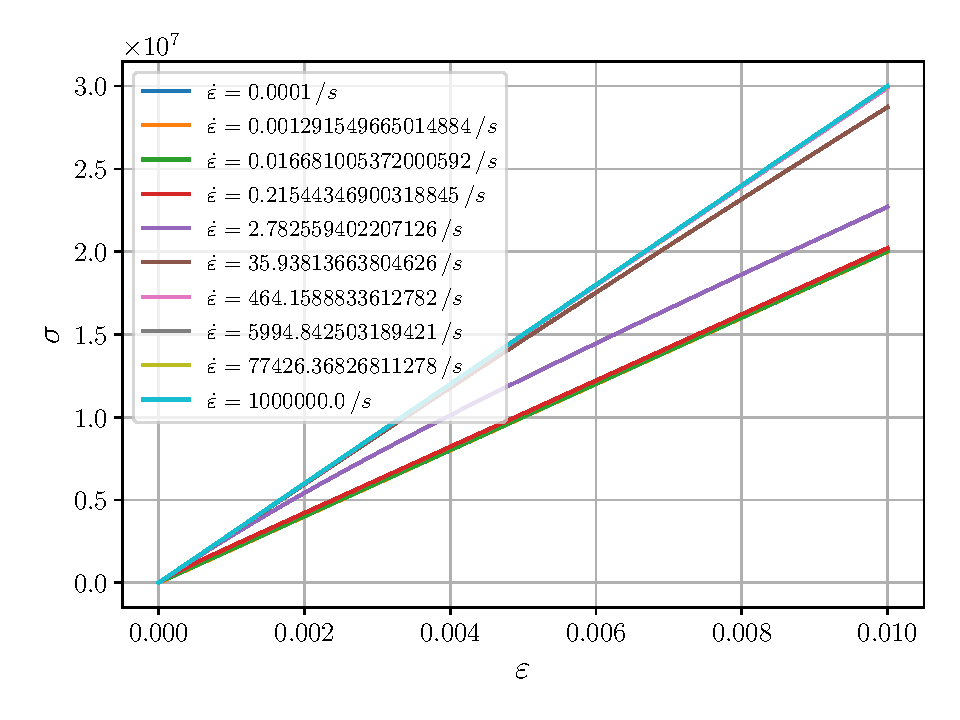
\includegraphics[width=\linewidth]{e-stress}
	\end{subfigure}
	\begin{subfigure}{0.48\textwidth}
		\centering
		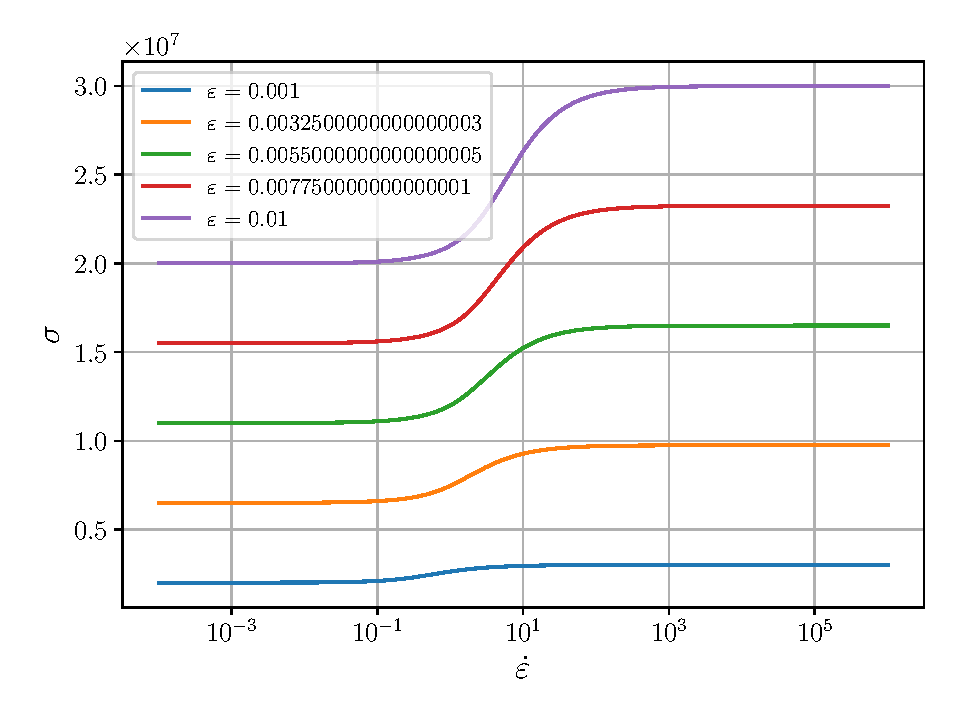
\includegraphics[width=\linewidth]{e-dot-stress}
	\end{subfigure}

	\begin{subfigure}{0.48\textwidth}
		\centering
		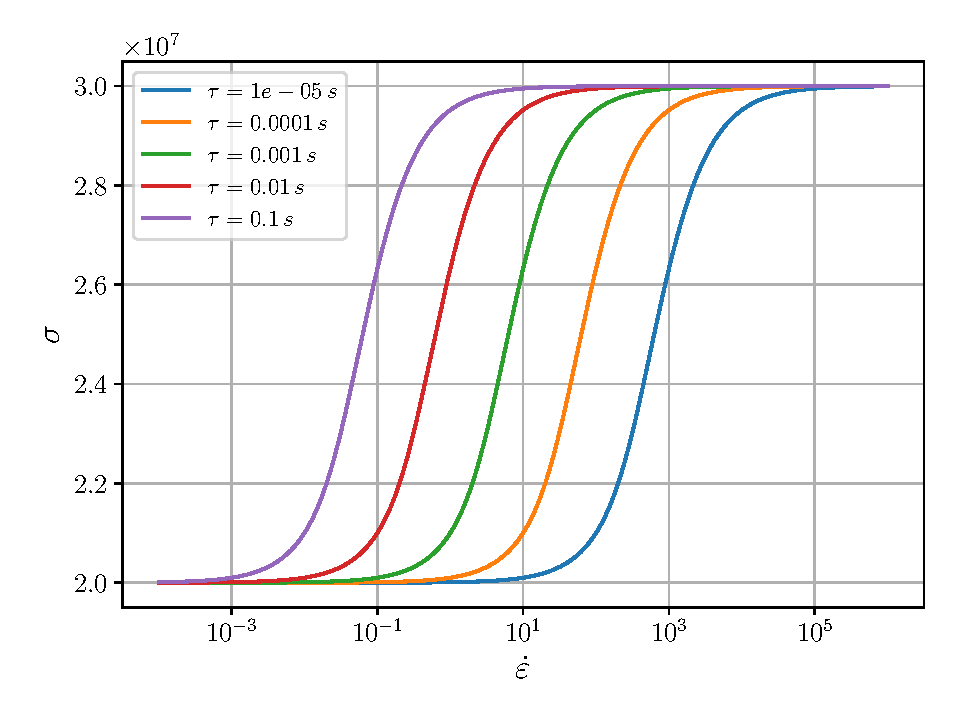
\includegraphics[width=\linewidth]{e-dot-stress-tau}
	\end{subfigure}
	\begin{subfigure}{0.48\textwidth}
		\centering
		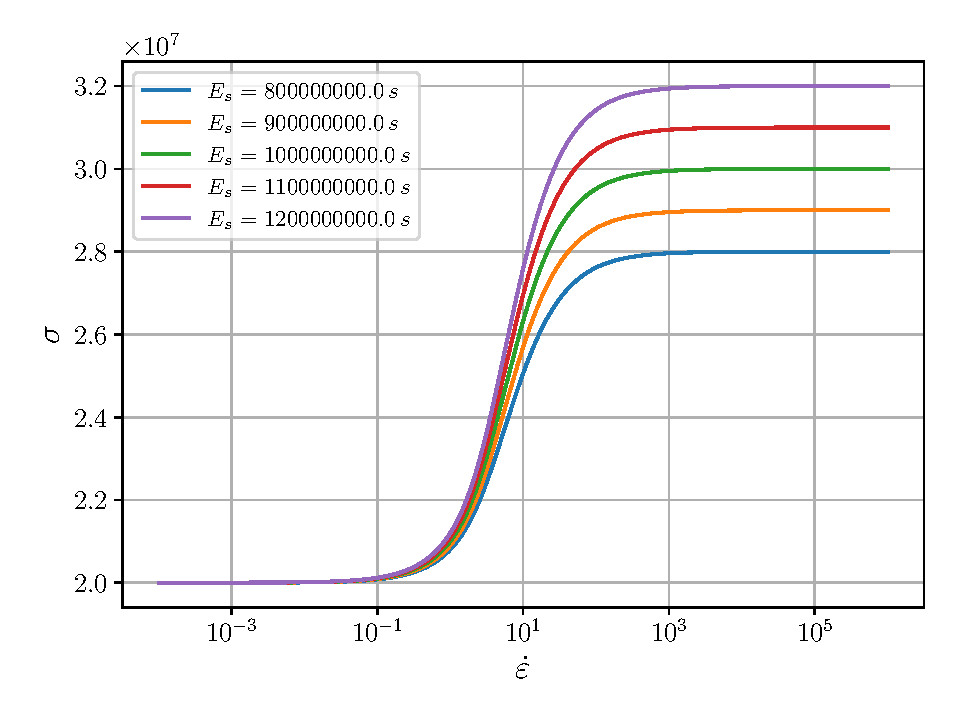
\includegraphics[width=\linewidth]{e-dot-stress-E}
	\end{subfigure}

\end{figure}

\subsection{Shear thickening and thinning models}

Bone is assumed to be impregnated with blood and other biological fluids which are susceptible to shear thinning or thickening

\begin{equation}
	\sigma^{d} = \eta(\dot{\epsilon}^{d})\dot{\epsilon}^{d}
\end{equation}

\begin{equation}
	\eta(\dot{\epsilon}^{d}) = K |\dot{\epsilon}^{d}|^{n-1}
\end{equation}

\end{document}
